
Nesta seção são descritas as etapas do projeto de um controlador por realimentação de estados para uma representação do sistema MIMO em espaço de estados. Inicialmente, é mostrada a conversão do sistema de FTs para espaço de estados, seguida da alteração das matrizes $C$ e $D$ para permitir a realimentação de todos os estados. Em seguida, são especificados os polos de malha fechada desejados e um controlador por realimentação de estados é obtido.

Inicialmente, obteve-se a matriz de FT do sistema MIMO, dada por:
$$ \begin{bmatrix}
        Y_{p}(s)\\
        Y_{Y}(s)\\
        \end{bmatrix} = \begin{bmatrix}
        G_{11} & G_{12}\\
        G_{12} & G_{22}\\
        \end{bmatrix}
        \begin{bmatrix}
        U_{1}(s)\\
        U_{2}(s)\\
        \end{bmatrix} $$

Em seguida, obteve-se sua representação em espaço de estados, obtendo-se
\begin{align*}
    \dot{x} &= A x + B u \\
    Y &= C x + D u
\end{align*}
\noindent onde
$$ A = \scalemath{0.92}{\begin{bmatrix}
        -0.2 & -2.1 & 0 & 0 & 0 & 0 & 0 & 0\\
        2 & 0 & 0 & 0 & 0 & 0 & 0 & 0 \\
        0 & 0 & -0.3 & -0.3 & 0 & 0 & 0 & 0 \\
        0 & 0 & 0.5 & 0 & 0 & 0 & 0 & 0 \\
        0 & 0 & 0 & 0 & -0.6 & -2.1 & 0 & 0 \\
        0 & 0 & 0 & 0 & 2 & 0 & 0 & 0 \\
        0 & 0 & 0 & 0 & 0 & 0 & -0.4 & -0.4 \\
        0 & 0 & 0 & 0 & 0 & 0 & 0.5 & 0 \\
        \end{bmatrix} }$$
        
$$ B = \begin{bmatrix}
        1 & 0 \\
        0 & 0 \\
        0.5 & 0 \\
        0 & 0 \\
        0 & 0.25 \\
        0 & 0 \\
        0 & 1 \\
        0 & 0 \\
        \end{bmatrix} $$

$$ C = \begin{bmatrix}
        0 & 0.95 & 0 & 0 & 0.19 & 0.05 & 0 & 0 \\
        0 & 0 & 0.6 & 0.07 & 0 & 0 & 0 & 0.7 \\
        \end{bmatrix} $$

$$ D = \begin{bmatrix}
        0 & 0 \\
        0 & 0 \\
        \end{bmatrix} $$

A resposta ao degrau do sistema em espaço de estados retornou o resultado mostrado na Figura \ref{fig:StepResponseEEModel}.

\begin{figure}[H]
    \centering
    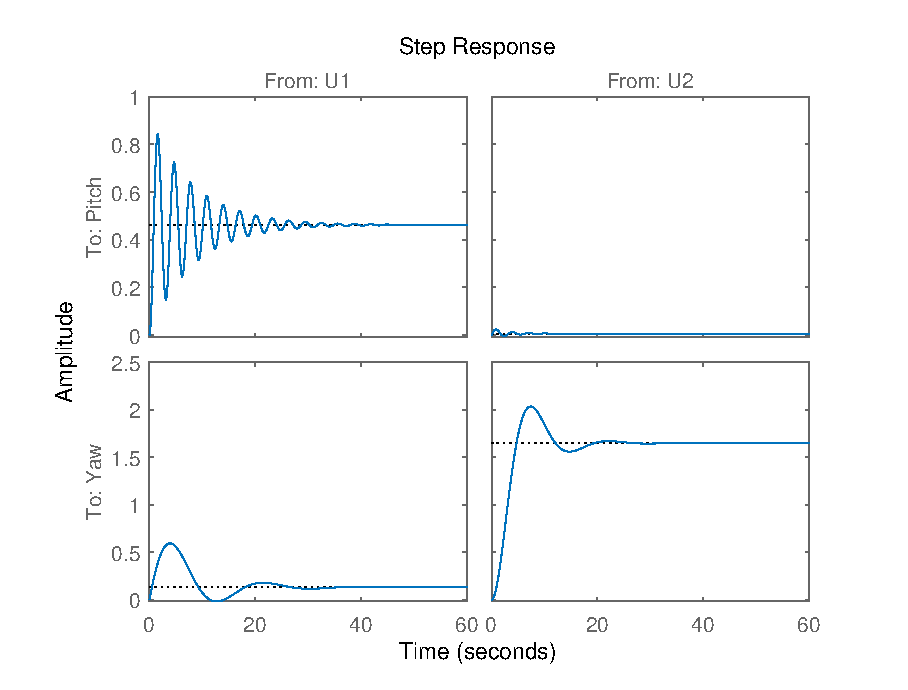
\includegraphics[width=0.48\textwidth]{figures/ControleEE/step_respons_ssmodel.eps}
    \caption{Resposta ao degrau do sistema MIMO em espaço de estados.}
    \label{fig:StepResponseEEModel}
\end{figure}

Um controlador por realimentação de estados requer que $u = - Kx$:
\begin{align*}
    \dot{x} &= A x - B k x \\
    \dot{x} &= (A - Bk) x
\end{align*}
\noindent onde $k$ representa uma matriz de ganhos da realimentação.

Para obtê-la, foram definidos os polos desejados de MF, segundo as especificações. Os quais foram obtidos pela ferramenta \textit{sisotool} do Matlab. A matriz de ganhos $k$ foi então obtida por meio do comando \textit{place()} do Matlab, passando-se as matrizes $A$ e $B$ e a matriz de polos desejados, obtendo-se

$$ k = \begin{bmatrix}
        3.12 & -0.15 & 0.01 & 0 & 0 & 0 & -0.06 & -0.18 \\
    0.15 & -0.03 & -0.2 & -0.04 & 0 & 0 & 2.9 & 6.8 \\
        \end{bmatrix} $$

Na Figura \ref{fig:StepResponseEEMAMF} é mostrada uma comparação entre a resposta do sistema MIMO a um degrau unitário em malha aberta e a resposta em malha fechada, a partir da realimentação de todos os estados com a matriz de ganho obtida.

\begin{figure}[h]
    \centering
    \includegraphics[width=0.48\textwidth]{figures/ControleEE/step_respons_allstates_MF_MA.eps}
    \caption{Resposta do sistema MIMO em MA e MF, considerando todos os estados da representação.}
    \label{fig:StepResponseEEMAMF}
\end{figure}

Para mapear de volta para as saídas desejadas, que relacionam o \textit{pitch} e o \textit{yaw} com as entradas $u_{1}$ e $u_{2}$, basta utilizar os ganhos presentes na matriz $B$.
